
In Just-In-Time scheduling, tardiness penalties typically dominate total objective costs because tight machine capacities propagate delays downstream across connected jobs.
While early operations can often be delayed to their target due dates without causing secondary delays, resolving tardiness requires expediting an entire chain of predecessor operations.
In classical Job Shop Scheduling for makespan minimization, the N5 neighborhood structure of \citet{nowicki1996fast} demonstrated that only reordering operations on the global critical path can shorten the makespan.
However, in JITJSS, the objective function does not depend on a single global critical path, but rather on the individual completion times of multiple operations with distinct due dates.
Consequently, classical makespan neighborhoods fail to address the specific precedence chains that produce tardiness penalties in JITJSS.

To address this challenge, we introduce a novel neighborhood operator, named \texttt{swap\_crit}.
The \texttt{swap\_crit} operator adapts the critical block concept to JITJSS by constructing an individual backward critical path for each tardy operation.
Let $u$ denote an operation that completes after its target due date ($C_u > d_u$).
To identify which operations actively delay $u$, the algorithm traces backward from $u$ along the disjunctive graph $G(\pi)$.
At each step, the algorithm identifies the bottleneck predecessor of an operation $v$ as whichever finishes latest between its job predecessor $JP[v]$ and machine predecessor $MP[v]$ (i.e., $\text{pred}^*(v) = JP[v]$ if $C_{JP[v]} \ge C_{MP[v]}$, and $MP[v]$ otherwise).
The algorithm prepends $\text{pred}^*(v)$ iteratively to the path until reaching an operation with no predecessors, yielding the individual critical path $P(u) = (v_1, v_2, \ldots, v_k = u)$ of operations whose completion times directly determine $C_u$.

\begin{figure}[!htbp] 
    \centering 
    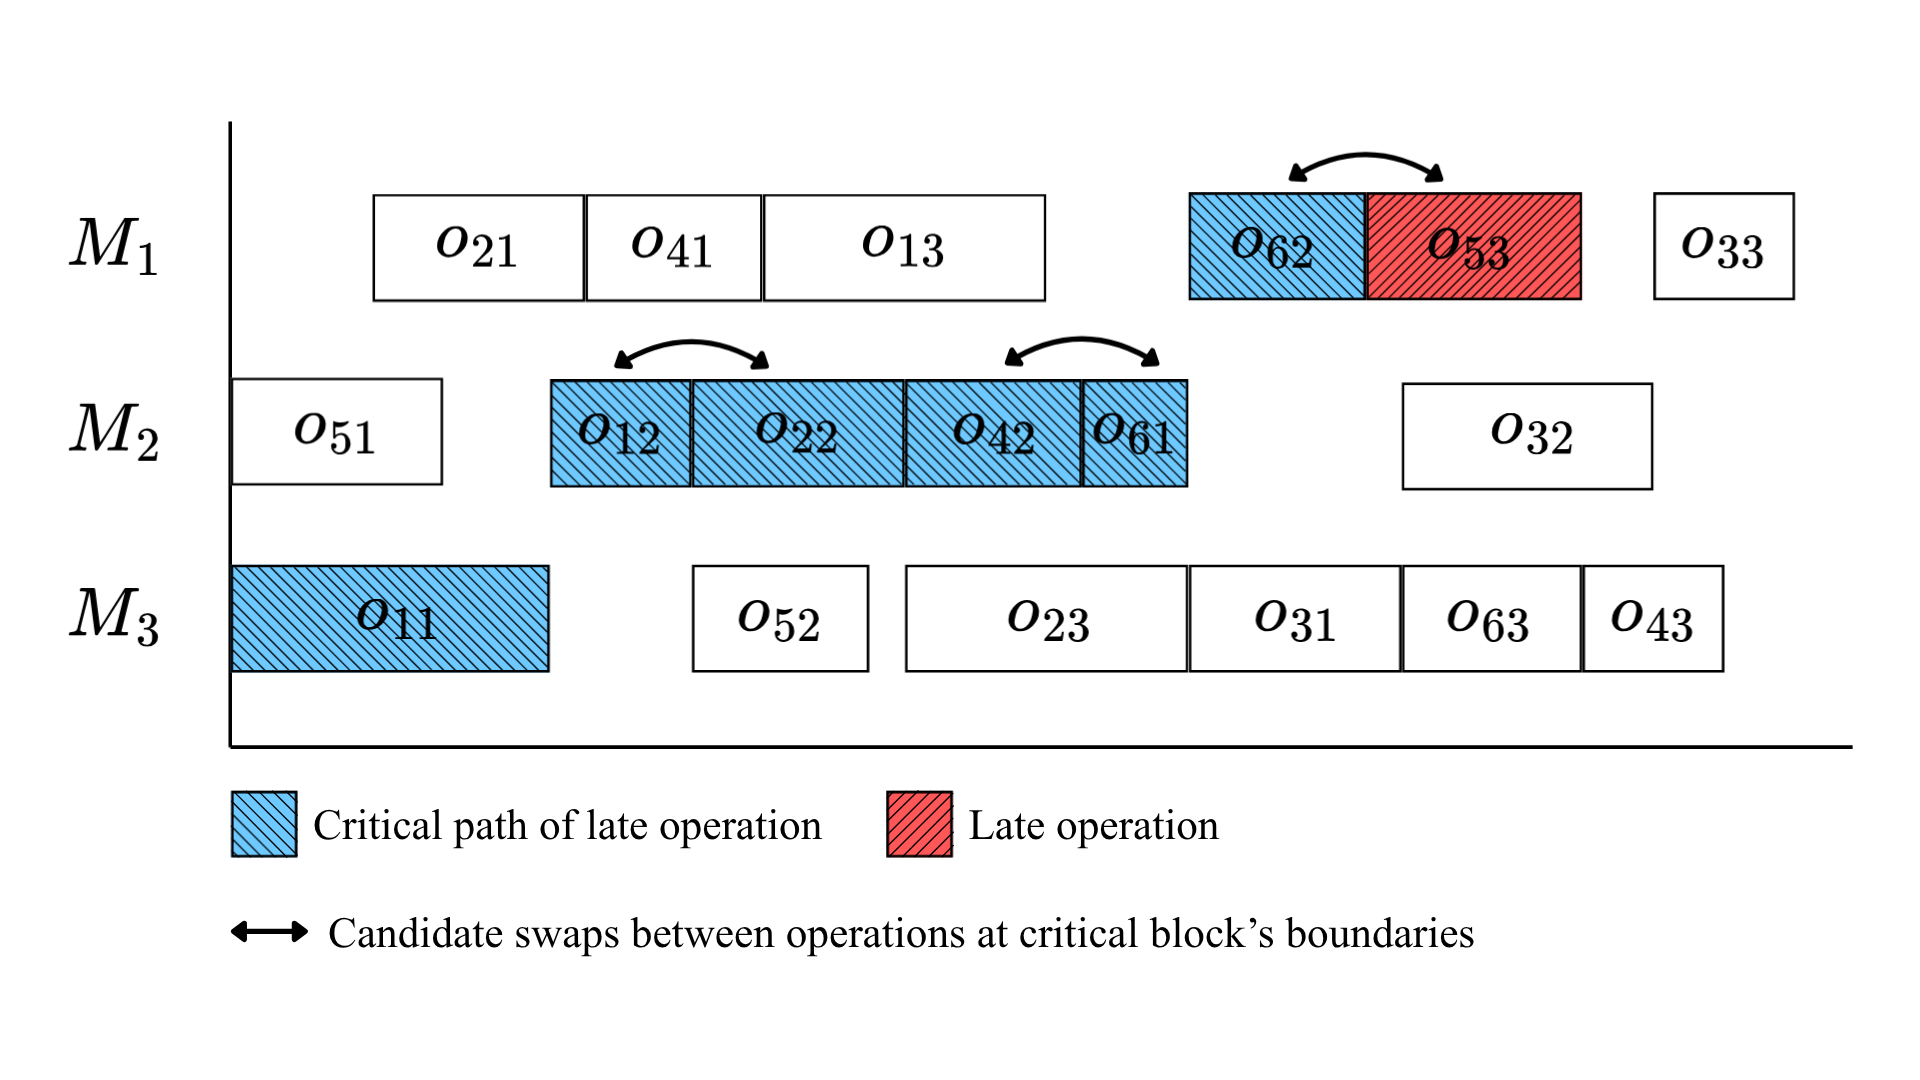
\includegraphics[width=0.75\linewidth]{img/oper_crit.png}
    %\caption{Example of individual critical-path tracing and candidate neighbor moves generated by the proposed \texttt{swap\_crit} operator.}
  \caption{\textbf{Critical block identification and candidate swap moves in the \texttt{swap\_crit} operator.} 
      Gantt chart illustrating the backward tracing of the critical path from a late operation $o_{53}$ (red hatched box). Operations belonging to its active critical chain are highlighted in blue. Candidate swapping moves are restricted strictly to adjacent operations located at the boundaries of critical blocks on each machine (indicated by double-headed arrows), avoiding internal non-improving permutations.}
    \label{fig:oper_crit}
\end{figure}

The algorithm then partitions $P(u)$ into maximal sub-sequences of consecutive operations processed on the same machine, termed \emph{critical blocks}:
\begin{equation}
B = (b_1, b_2, \ldots, b_q), \quad q \ge 2
\end{equation}
Because internal swaps cannot shorten the critical path \citep{nowicki1996fast}, \texttt{swap\_crit} only swaps operations at block boundaries:
\begin{enumerate}[(i)]
    \item If $|B| = 2$, the operator swaps the two operations $(b_1, b_2)$.
    \item If $|B| \ge 3$, the operator generates two distinct candidate moves: swapping the first two operations $(b_1, b_2)$ and swapping the last two operations $(b_{q-1}, b_q)$.
\end{enumerate}

Figure~\ref{fig:oper_crit} illustrates this process on an exemplary schedule where operation $o_{53}$ is tardy ($C_{53} > d_{53}$).
Tracing backward from $o_{12}$ yields the individual critical path $o_{11} \to o_{12} \to o_{22} \to o_{42} \to o_{61} \to o_{62} \to o_{53}$.
Along this path, consecutive operations sharing the same machine form critical blocks.
Applying the boundary swap rules generates three candidate neighbor solutions: swapping $o_{12}$ with $o_{22}$, swapping $o_{42}$ with $o_{61}$, and swapping $o_{62}$ with $o_{53}$.
By altering these precedence constraints, each candidate move can directly advance the start time of $o_{53}$ and reduce its tardiness.

